\chapter{Extensions to the Neural Engineering Framework}
\label{chapt:nef-extensions}


\section{Challenges Posed by Neuromorphic Hardware}

Some of these are already solved to some extent by standard NEF. Others require more careful consideration / theoretical extensions.

\subsection{Discretization}

\subsection{Quantization}

\subsection{Connectivity}

\subsection{Memory}

Weight factorization on SpiNNaker, Braindrop, and Loihi

\subsection{Spike Traffic}

Amount of internal traffic.

\subsection{External Input-Output}

Amount of external traffic. Also encoding the inputs as spikes, and decoding the outputs.

\subsection{Thermal Variation}

\subsection{Transistor Mismatch}

\subsection{Digital to Analog Conversion}

Pulse-extender

\subsection{Higher-Order Dynamics}

Special case of transistor mismatch


\section{Arbitrary Linear Synapses}

Insert patent here.

\subsection{Linear Transfer Function Characterization}

\subsection{Nonlinear State-Space Characterization}

\subsection{Time-Constant Mismatch}

\subsection{Encoding Filters}

This section is taken from \citep{voelker2016a}.

Giving robots the ability to classify surface textures requires appropriate sensors and algorithms. Inspired by the biology of human tactile perception, we implement a neurorobotic texture classifier with a recurrent spiking neural network, using a novel semi-supervised approach for classifying dynamic stimuli. Input to the network is supplied by accelerometers mounted on a robotic arm. The sensor data is encoded by a heterogeneous population of neurons, modeled to match the spiking activity of mechanoreceptor cells. This activity is convolved by a hidden layer using bandpass filters to extract nonlinear frequency information from the spike trains. The resulting high-dimensional feature representation is then continuously classified using a neurally implemented support vector machine. We demonstrate that our system classifies 18 metal surface textures scanned in two opposite directions at a constant velocity. %In particular, the system correctly classifies 65.6\% of all 1 second test recordings. 
We also demonstrate that our approach significantly improves upon a baseline model that does not use the described feature extraction. 
This method can be performed in real-time using neuromorphic hardware, and can be extended to other applications that process dynamic stimuli online. 

Humans are remarkably adept at perceiving the environment using their sense of touch. By moving the fingertip across a surface, vibrations give rise to perceptual qualities such as roughness \citep{unger2013physical}, stickiness, and slipperiness \citep{klatzky2013haptic, holliins1993perceptual}. Thus, structural details smaller than 1\,\si{\micro\meter} in different quality grades of silk, paper, and grind metal surfaces can be differentiated \citep{weber2013spatial}.
%, smaller than the distance between specialized mechanoreceptors within the fingertip.
%It is made possible by mechanoreceptors innervating our skin which are sensitive to dynamic stimuli, namely vibrations. These origin from the contact area between skin and texture when moving the finger \citep{weber2013spatial}. 
%The relationship, however, is highly on-linear and complex. In the case of texture classification, the challenge lies within finding distinctive features in these vibration patterns. %The challenge  is to find physical quantities which can be linked to perceptual qualities. 
Our goal is to draw inspiration from nature to give robots the ability to classify surface textures in real-time. This ability can be deployed within systems that need to classify tactile stimuli, such as those employed to automate quality control of textured surfaces. 


Dynamic robotic systems for tactile surface sensing have been developed using various technologies \citep{dahiya2010tactile}. In this context, \textit{tactile} implies the sensors physically touch the textured surface. \textit{Dynamic} refers to robotic setups that perform exploratory movements across the surface to accumulate sensor data. % Sensing technologies - Accelerometers
Accelerometers have been used as dynamic vibration sensors for texture discrimination in %\citep{howe1989sensing} 
\citep{howe1993dynamic}, \citep{giguere2011simple} %(mems acc on flexible probe)
and \citep{sinapov2011vibrotactile}. 
By using only the signal variance of two spatially separated vibration sensors, four different textures could be differentiated in \citep{tada2004sensing}. In addition to variance, Giguere and Dudek \citep{giguere2011simple} utilized mean, skewness, kurtosis and some higher order moments of one accelerometer to differentiate between ten fine and coarse textures. 
Other studies have used multiple exploratory movements to boost classification accuracy. For instance, Sinapov et al. \citep{sinapov2011vibrotactile} used five exploratory movements with varying direction and speed, and analyzed the spectrotemporal features to classify twenty naturalistic fine textures with $80\%$ accuracy. Another study kept executing exploratory movements until at least $80\%$ of the movements indicated a specific texture \citep{jamali2011majority}.


% 2. Data processing and exploratory movement
% Systems using different sensors but interesting in terms of data processing: \citep{oddo2011roughness} SSSA biotact sensor using mems pressure sensing, 

However, only a few groups have developed classifiers using spiking neural networks. A closed perception-action loop was built to classify Braille characters \citep{bologna2013closed}, by supplying pressure sensor array data to {\it leaky integrate-and-fire} (LIF) 
neurons, and then using a naive Bayes classifier to control the scanning velocity. 
Another approach classified ten naturalistic textures with $97\%$ accuracy \citep{rongala2015neuromorphic}, by simulating an Izhikevich neuron in response to an array of four piezoresistive sensors, and analyzing the precise spike timing using spike distance metrics. However, these metrics require offline processing of the entire time window, and therefore cannot be implemented in real-time.

% Jeremy Fishel - Bayesian exploration
Related work has also used {\it Bayesian exploration} to optimize the information supporting various textural \mbox{properties \citep{fishel2012bayesian}}. This model is capable of using a number of exploratory movements to classify $117$ textures with a $95.4\%$ success rate. However, the system requires an offline phase to reduce the input signal to a number of scalar values, making it unsuitable for real-time applications. This reduction could also discard valuable information from the input signal, since it is manually crafted using a finite set of properties motivated by psychophysical studies. 

In contrast, we find it possible to automatically discover the most salient {\it features} from a high-dimensional representation of the input stimulus, %and process this signal to extract 
and classify these features {\it online}.  This is challenging since the relationship between a rapidly time-varying tactile stimulus and its resulting perceptual qualities is highly nonlinear \citep{weber2013spatial}. To make this problem tractable, we translate our biological understanding of tactile perception into an artificial network  of spiking neurons, and then train the desired function. Our approach  % from the mechanoreceptors to the classification result
is implemented entirely within a spiking neural network that can be simulated on low-power neuromorphic hardware. 

%As opposed to \citep{jamali2011majority}, we only use data gathered from one type of exploratory movement at one fixed velocity. 
%

When fingers move across a texture, tiny hills and valleys along its surface rapidly excite various types of static and dynamic {\it mechanoreceptors} \citep{weber2013spatial}. Biomechanical processes within these cells convert the physical forces applied by the stimulus into spike trains. We adapt a mechanoreceptor model by Kim et al. \citep{kim2011does} to simulate this process in a population of spiking neurons.  The nervous system routes the mechanoreceptor responses  through the spinal cord where they are  processed by cuneate neurons \citep{saal2014touch}, which function as feature extractors across this spiking activity   \citep{jorntell2014segregation}. This motivates the inclusion of a {\it hidden layer} in the model  to extract a high-dimensional feature representation. We have designed  this layer to encode frequency bands of the stimulus, since frequency is an important factor in psychophysical experiments involving the differentiation of textures \citep{unger2013physical}. 
The population of cuneate neurons project these features to somatosensory cortex, where an abstract percept of the texture is thought to be formed  \citep{jorntell2014segregation}. Our model  learns the mapping from features to textures using a support vector machine (SVM). These learned weights are embedded  within the connection to a recurrent output layer. To summarize, the network encodes the physical stimulus into spiking activity, maps this activity to extract salient features, and finally decodes the resulting spikes to obtain an online classification. 

To implement this model, we employ  the Neural Engineering Framework (NEF), which  provides a method for mapping functions to a biologically plausible spiking neural network \citep{eliasmith2003a}. %This provides our system with a number of unique advantages that advance the field of robotics. 
These networks can be efficiently simulated on neuromorphic hardware such as SpiNNaker \citep{mundy2015}, resulting in significant energy savings \citep{hasler2013finding}. Simulations are also more efficient than all-to-all connected networks due to the use of factored weight matrices \citep{bekolay2013},  and are generally robust to noise and physical variability due to heterogeneity \citep{hunsberger2014}.

Our method uses the NEF to classify surface textures scanned with a robotic setup. We report performance on a set of 18 metal surface textures. This establishes a novel biologically-inspired system that can be simulated in real-time using neuromorphic hardware.

\subsubsection{Mechanoreceptor Model}

\newcommand{\gammafactor}{\mbox{\it $\Gamma$-factor} (GF)}

The human sense of touch uses free nerve endings and specialized mechanoreceptors to sense vibrations on the skin. The latter are composed of two types: 1) slowly adapting type cells which are sensitive to static stimuli; 2) the so-called rapidly adapting type cells. The slowly adapting cells include Merkel (SA1, static pressure) and Ruffini cells (SA2, skin stretch). The rapidly adapting cells are sensitive to transient events such as vibration. These include Meisser (RA, vibration in the range of 1 to about 60\,Hz) and Pacinian cells (PC, vibrations in the range of 30 to about 700\,Hz) \cite{johansson2009coding}. When the finger moves across a surface texture, the skin is excited by vibration patterns influenced by macro- and microscopic topography of the surface in contact. These cells transform the physical stimulus into spiking patterns.

%% Description of the mechanoreceptor population model%%
To mimic this biological representation, our model encodes the vibrations recorded from multiple accelerometers into the spiking activity of a heterogeneous population of mechanoreceptor neuron models.  Since SA2 cells do not contribute directly to fine textural percepts \cite{weber2013spatial}, we only consider PC,  RA, and SA1 type cells for our model. 

%% Description of the individual receptor principle%%

The mechanoreceptor model by Kim et al. \cite{kim2011does} has been shown to accurately reproduce the spike trains of RA and SA1 type cells on a variety of stimuli.  Following this model, we take the acceleration $u(t)$, and its two derivatives $\dot{u}(t)$, $\ddot{u}(t)$, and separate each of them into positive and negative rectified parts resulting in $6$ signals. % We may interpret $u(t)$ as the applied to the fingertip, since force is proportional to acceleration. 
Since acceleration is directly proportional to the net force, we interpret $u(t)$ as the force applied to the fingertip.
Then $\dot{u}(t)$ and $\ddot{u}(t)$ are the first- and second-order changes in force, respectively.  As shown in \mbox{Fig. \ref{fig:touch-network}}, the rectified signals form 6 inputs, which are weighted and summed to form the current to an adaptive LIF neuron.
%As shown in Fig. \ref{fig:netw_struct}, these 6 signals are weighted and summed to form the input current to an adaptive LIF neuron.

This is equivalent to the neural representation of a $6$-dimensional vector $\V{x}(t)$ in the NEF using (\ref{eq-neuron}). Each encoding vector $\V{e}_i$ corresponds to the $6$ weights that depend on the cell type of the $i^{th}$ neuron. Different weights then reproduce the spiking characteristics of different types of mechanoreceptors.  For the PSC model required by the NEF, we use a lowpass filter with time constant $\tau = 1$\,ms on all mechanoreceptors. We found experimentally that this constant works well to balance the need for smoothing (large $\tau$) with the need to maintain high frequencies in the signal (small $\tau$).  To simplify implementation, differentiation is performed by combining this PSC filter with a highpass filter with the same time constant (Laplace transform $\tau s$). Our model differs from the original model only by  the use of an adaptive LIF model instead of the {\it Mihalas-Niebur} model, and by omitting a saturation filter applied to the current. The adaptive LIF model is used in place of $G[\cdot]$ to obtain a neural model that is simpler than Mihalas-Niebur while still supporting adaptation. We then use (\ref{eq-neuron}) to simulate the spiking activity of each neuron in response to the stimulus.

\begin{figure}[!tbp]
    \centering
    \vspace{-2pt}
    \includegraphics[width=0.49\textwidth]{touch-1}
     
    \caption{\label{fig:touch-network} Architecture of the surface texture classifier. Data from three sensors are encoded in the spiking activity of mechanoreceptor neurons. A hidden layer extracts nonlinear features of these spike trains in the frequency domain by convolution with bandpass filters. A recurrently connected output (feedback arrows omitted) represents the score for each class, smoothed over time. This score vector is linearly decoded from the recurrent layer to find the texture with the largest score. Connection weights and neural parameters  are given by the principles of the NEF.}
\end{figure}

Rather than fitting the parameters of the neurons directly to individual model neurons  as in the original model, we uniformly randomize parameters $\alpha_i$, $\beta_i$, and $\V{e}_i$ of $\numprint{40000}$ neurons (this number was chosen to sufficiently sample the space of parameters), and then select those with the highest \gammafactor{} \cite{jolivet2008benchmark} to canonical PC/RA/SA1 models on a standard test stimulus\footnote{Canonical models and test data were obtained by email correspondence with the authors of \cite{kim2011does}. Although PC type cells were not evaluated by the original study, their model included sample PC parameters.}
The GF compares the number of coincidental spikes within a $\pm 2$\,ms window to the expected value generated by a Poisson process with the same firing rate: $1$ implies a perfect match; $0$ a Poisson process; and $-1$ indicates anti-correlation. We use this particular measure to be consistent with the  prior analysis of the original model. %Thus we assure biological realism of the selected populations. 
The pruned population of mechanoreceptors contains $20/300/200$ neurons ($520$ total)  of type PC/RA/SA1, respectively, to match the distribution within a $2$\,cm$^2$ % should cm be italicized?
surface of contact \cite{johansson2009coding}. % Around $0.5\%$ of the total neurons had a \gammafactor{} exceeding $0.8$ with at least one of the canonical PC/RA/SA models.
The GF of selected neurons range from $0.19$ to $0.99$  with mean $0.49$ across all three types. This is promising considering Kim et al. \cite{kim2011does} found the mean GF between individually fit models and their canonical RA/SA1models to be approximately $0.3$.

The resulting distribution of encoders effectively reflects the sensitivity of each cell to various characteristics of the sensory input. By allowing them to vary randomly, the information content of the population is increased \cite{hunsberger2014}. In particular, the network can further process the $6$-dimensional representation using (\ref{eq-decoder})  while being robust to noise.
This need to exploit individual variability is consistent with the conclusion made by Kim et al. \cite{kim2011does} that heterogeneity in afferent fibers matters when conveying precise timing information about the tactile response.

The fingertip has multiple points of contact while scanning a surface, allowing it to pick up spatial features of the stimulus \cite{weber2013spatial}. The above $6$-dimensional encoding is repeated 3 times (for each sensor in our robotic setup)  to form an $18$-dimensional representation, where the encoding vector for each neuron is tuned to different combinations of dimensions from the different sensors. This further improves robustness to noise by exploiting multiple correlated sources of information. %, and effectively permits the neural representation to exploit any nonlinear interactions between sensors. 
The distribution of encoders could also be controlled to match known spatial characteristics of each cell, but for simplicity we set all encoders to be uniformly distributed across the 3 sensor signals.

\subsubsection{Dynamical Feature Extraction}

Given the spiking activity of the population of mechanoreceptors, we now extract a high-dimensional representation in a hidden layer of neurons,  to capture general features of the stimulus.

The $18$-dimensional input representation ($6$ dimensions $\times$ $3$ sensors) is recovered from the spiking activity of the mechanoreceptor population,  by solving (\ref{eq-decoder}) for a $520 \times 18$ decoder matrix $\V{d}$ ($18$ input dimensions for each of the $520$ mechanoreceptor neurons)  using regularized least squares optimization. The parameters of $\numprint{7200}$ LIF neurons (this number was chosen to sufficiently sample the space of neural parameters per dimension), one for each feature in the hidden layer,  are randomly generated, with encoders constrained to each of the possible $18$ dimensions. This forms a sparse $\numprint{7200} \times 18$ encoder matrix $\V{e}$ such that (\ref{eq-conn}) gives the connection weight matrix from the mechanoreceptor population to the hidden layer. % the sparsity reduces time/space by a factor of 18 -- and the number of neurons in this layer is reduced in section \ref{sec_classifier}.
The hidden layer then represents the same $18$-dimensional input at the current point in time, by having learned the optimal decoding from the spikes of the adaptive mechanoreceptor layer. 

Motivated by the importance of stimulus frequency in psychophysical experiments involving texture \mbox{discrimination \cite{unger2013physical}}, our aim is to extract features that encode information about the frequency of the current stimulus.  The weight matrix transforms the activity independently of time, and is therefore insufficient to extract information about its frequency content. Thus, we provide the $i^{th}$ neuron in the hidden layer with its own PSC filter $h_i(t)$, modeled as a {\it $2^{nd}$ order bandpass} filter with Laplace transform
\begin{equation}
\label{eq-bandpass}
H_i(s) = \frac{1}{\frac{1}{\omega_i^2}s^2 + \frac{1}{\omega_i Q_i}s + 1}
\end{equation}
where $\omega_i$ is the peak frequency in radians per second, and $Q_i$ is inversely proportional to the bandwidth. This filter was chosen because it is the linear filter of lowest order that is capable of isolating particular bands of frequencies. 

Each $\omega_i$ %(or $2 \pi f$, where $f$ is the frequency in Hertz) 
is chosen randomly without examining the input data. Since differentiation is a form of highpass filtering, we expect the higher derivatives to represent higher frequency bands more accurately. Thus $\omega_i$ is chosen between $0 - 250$, $125 - 375$, or $250 - 500$\,Hz, depending on whether the neuron is encoding a dimension from $u(t)$, $\dot{u}(t)$, or $\ddot{u}(t)$, respectively. Frequencies above $500$\,Hz are unnecessary due to the refractory rates of neurons ($2$\,ms). We found that randomizing $Q_i$ between $2 - 50$, regardless of dimension, lead to the best results. 

The spiking activity of each hidden neuron encodes a recovered input dimension convolved with a random bandpass filter (see Fig. \ref{fig:netw_struct}). Decoding the square of a particular filter from this population then yields the power of that filter. More generally, any nonlinear functions of the frequency bands that are supported by the neural basis functions\footnote{Eliasmith and Anderson \cite{eliasmith2003a} characterize this in detail using singular value decomposition on the activity matrix, and show that squaring is accurately supported by LIF tuning curves.} can be used as a feature -- a fact readily exploited in  the following subsection.

\subsubsection{Recurrent Classification}

\newcommand{\outputNeurons}{900}

The final layer of our model is a recurrent output layer,  which classifies the spiking activity of the hidden layer into one of $k$ possible surface textures. The output layer is a population of $\outputNeurons{}$ LIF neurons that represent a $k$-dimensional vector %(using (\ref{eq-neuron}) and (\ref{eq-decoder})) 
encoding a {\it score} for each class. The value of $\outputNeurons{}$ was chosen to be large enough to accurately decode all $k$ dimensions using (\ref{eq-decoder}).

Since the activity of the hidden layer is noisy and high-dimensional, we use scikit-learn (v0.16.1) to train a {\it one-vs-all linear support vector machine} (SVM), from the spikes of the hidden layer, without being prone to overfitting  \cite{pedregosa2011scikit}. Since each of the $k$ classifiers  computes a dot product, together they form a $\numprint{7200} \times k$ decoder matrix $\V{d}$ (one decoding vector for each neuron in the hidden layer)  equivalent to solving (\ref{eq-decoder}) using the SVM maximum margin objective.

A $\numprint{\outputNeurons{}} \times k$ encoder matrix $\V{e}$ (one encoding vector for each neuron in the output layer)  is randomly generated, and (\ref{eq-conn}) provides the weight matrix to the output layer. To determine the resulting classification, we again solve for a $\numprint{\outputNeurons{}} \times k$ decoder matrix $\V{d}$, so that (\ref{eq-decoder}) produces an estimate of the $k$-dimensional score vector. The index of the maximum value yields the classification for the given point in time. 

The population is recurrently connected to itself using (\ref{eq-leaky}) to integrate the scores with a leak term. This smooths the classification over time, with different recurrent lowpass time constants ($\tau_0$) altering the rate of adaptation to new stimuli or the forgetting of old evidence. We use $\tau_0 = 50$\,ms  and \mbox{$\tau = 5$\,ms} for the output layer. The value of $\tau$ matches the default synaptic time-constant in our simulation software, while $\tau_0$ was found to help persist correct classifications over time intervals with insufficient evidence in the signal. 

It is important to note that although the SVM itself is linear, its features are not, due to the neural nonlinearities in the hidden layer. This is mathematically equivalent to using a kernel function given by the LIF tuning curves. %This provides the SVM with a rich set features that are nonlinear in the encoded frequencies%
Thus, the SVM nonlinearly separates the encoded frequency bands using randomly generated neural basis functions.

\subsubsection{Software}

All experiments were run using Nengo (v2.0.1), a Python implementation of the NEF \cite{bekolay2013nengo}. Neurons were configured with default parameters, and the parameters from (\ref{eq-neuron}) were randomly sampled across the default ranges. Nengo automatically learned the decoders and connection weights offline, by optimizing the RMSE of (\ref{eq-decoder}) given randomly sampled $\V{x}(t)$ from the unit hypersphere.

The simulations of (\ref{eq-neuron}) used a timestep of $0.5$\,ms ($2$\,kHz). % ($0.2$ times the data sampling rate). -- data sampling rate has not been mentioned yet
The accelerometer data $u(t)$ was streamed as input to the neural network. The spike train of the output population was read to obtain a classification at each timestep. %We now proceed with details of the architecture in Nengo within the context of the NEF.

Details of the experimental setup may be found in \citet{voelker2016a}.

\subsubsection{Results}

\begin{figure}[!htb]
    \centering
    \vspace{1pt}
    \includegraphics[width=0.4\textwidth]{touch-4}
    \caption{\label{fig:touch-raster} Network activity on a $1$ second test segment from the S2.5 %(face milling, $2.5$\,Rz) 
recording. (Top) Normalized accelerometer data from the three sensors, across an interval of $0.2$ to $0.4$\,s. (Middle) Spike raster of 15 (out of 520) randomly selected mechanoreceptor neurons, over this same time interval. (Bottom) Top 4 scores across the entire $1$\,s segment, obtained by decoding the output population. The network correctly classifies the texture as S2.5 at every timestep after the first $10$\,ms.
}
\end{figure}

\begin{table*}[!htbp]
    \centering
    \vspace{5pt}
    \caption{\label{tab:touch-results} Confusion Matrix for $1$\, Second Test Segments (\%) }
    \renewcommand{\arraystretch}{1.1}  % stretch vertical padding to make the table appear cleaner
    \renewcommand{\tabcolsep}{0.195cm}  % squish horizontal padding to avoid overflowing into margins
    \tiny
\begin{tabular}{ | c c || c c c c c c c c c c c c c c c c c c | } \hline & &  \multicolumn{18}{c|}{\bf Predicted} \\ & & F.55 & F1 & F1.6 & H2.5 & H4 & H8 & L2.5 & L4 & L8 & S2.5 & S4 & S8 & P.55 & P1 & P1.6 & G3 & G6 & G10 \\ \hline \hline \multirow{18}{*} {\rotatebox[origin=c]{90}{\bf Actual}} & F.55 & {\bf 96.7} & 0.8 & 0.0 & 0.0 & 0.0 & 0.0 & 0.8 & 0.0 & 0.0 & 0.0 & 0.0 & 0.0 & 0.0 & 0.0 & 0.0 & 0.8 & 0.0 & 0.8 \\ & F1 & 14.2 & {\bf 55.8} & 8.3 & 0.0 & 0.0 & 0.0 & 0.0 & 0.0 & 0.0 & 0.0 & 0.0 & 0.0 & 0.8 & 9.2 & 0.0 & 4.2 & 1.7 & 5.8 \\ & F1.6 & 4.2 & 0.0 & {\bf 80.0} & 0.0 & 0.0 & 0.0 & 0.8 & 2.5 & 1.7 & 0.0 & 1.7 & 0.0 & 0.0 & 7.5 & 0.0 & 0.8 & 0.0 & 0.8 \\ & H2.5 & 0.8 & 0.0 & 1.7 & {\bf 40.8} & 0.0 & 5.8 & 0.0 & 0.0 & 0.8 & 5.0 & 33.3 & 1.7 & 8.3 & 0.0 & 0.8 & 0.0 & 0.0 & 0.8 \\ & H4 & 0.0 & 0.0 & 0.0 & 0.0 & {\bf 99.2} & 0.0 & 0.0 & 0.0 & 0.0 & 0.0 & 0.0 & 0.0 & 0.8 & 0.0 & 0.0 & 0.0 & 0.0 & 0.0 \\ & H8 & 0.0 & 0.0 & 0.0 & 0.0 & 1.7 & {\bf 68.3} & 0.0 & 0.0 & 1.7 & 1.7 & 9.2 & 1.7 & 10.0 & 1.7 & 0.0 & 0.0 & 0.8 & 3.3 \\ & L2.5 & 4.2 & 0.0 & 4.2 & 0.0 & 0.0 & 0.0 & {\bf 73.3} & 0.8 & 7.5 & 6.7 & 2.5 & 0.0 & 0.0 & 0.0 & 0.0 & 0.8 & 0.0 & 0.0 \\ & L4 & 0.0 & 0.0 & 10.0 & 0.0 & 0.0 & 0.0 & 2.5 & {\bf 60.0} & 0.0 & 0.0 & 25.0 & 0.8 & 0.8 & 0.0 & 0.8 & 0.0 & 0.0 & 0.0 \\ & L8 & 3.3 & 0.0 & 10.8 & 0.0 & 0.0 & 0.8 & 16.7 & 8.3 & {\bf 49.2} & 0.0 & 1.7 & 0.8 & 3.3 & 0.8 & 0.0 & 2.5 & 0.0 & 1.7 \\ & S2.5 & 0.0 & 0.0 & 0.0 & 0.8 & 0.0 & 10.8 & 5.0 & 0.0 & 2.5 & {\bf 67.5} & 0.8 & 0.0 & 5.0 & 0.0 & 0.0 & 6.7 & 0.8 & 0.0 \\ & S4 & 0.0 & 0.0 & 0.8 & 0.0 & 0.0 & 0.0 & 0.0 & 1.7 & 0.8 & 1.7 & {\bf 92.5} & 0.0 & 0.0 & 0.8 & 1.7 & 0.0 & 0.0 & 0.0 \\ & S8 & 0.0 & 0.8 & 0.8 & 0.8 & 0.0 & 9.2 & 1.7 & 0.0 & 0.8 & 14.2 & 17.5 & {\bf 40.0} & 0.8 & 1.7 & 6.7 & 0.0 & 0.0 & 5.0 \\ & P.55 & 0.8 & 0.0 & 0.8 & 0.8 & 0.0 & 7.5 & 0.0 & 0.0 & 0.8 & 0.0 & 2.5 & 0.0 & {\bf 75.0} & 5.8 & 0.0 & 4.2 & 0.0 & 1.7 \\ & P1 & 0.8 & 0.0 & 1.7 & 0.0 & 0.0 & 5.0 & 0.0 & 0.8 & 0.0 & 0.0 & 2.5 & 0.0 & 10.8 & {\bf 55.8} & 0.0 & 6.7 & 0.8 & 15.0 \\ & P1.6 & 0.0 & 0.0 & 0.0 & 0.8 & 0.0 & 0.8 & 0.0 & 0.8 & 0.8 & 0.0 & 0.8 & 0.0 & 0.0 & 0.0 & {\bf 95.8} & 0.0 & 0.0 & 0.0 \\ & G3 & 10.0 & 0.0 & 2.5 & 0.0 & 0.0 & 2.5 & 0.0 & 0.0 & 0.0 & 17.5 & 0.0 & 0.0 & 4.2 & 7.5 & 1.7 & {\bf 41.7} & 7.5 & 5.0 \\ & G6 & 10.0 & 6.7 & 2.5 & 0.0 & 0.8 & 4.2 & 0.8 & 0.0 & 0.0 & 1.7 & 3.3 & 0.0 & 1.7 & 5.8 & 2.5 & 25.8 & {\bf 29.2} & 5.0 \\ & G10 & 0.0 & 0.0 & 10.0 & 0.0 & 1.7 & 0.8 & 1.7 & 0.0 & 2.5 & 0.0 & 3.3 & 0.0 & 0.8 & 18.3 & 0.0 & 0.8 & 0.0 & {\bf 60.0} \\ \hline \end{tabular}
\end{table*}

\begin{figure}[!htb]
    \centering
    \vspace{5pt}
    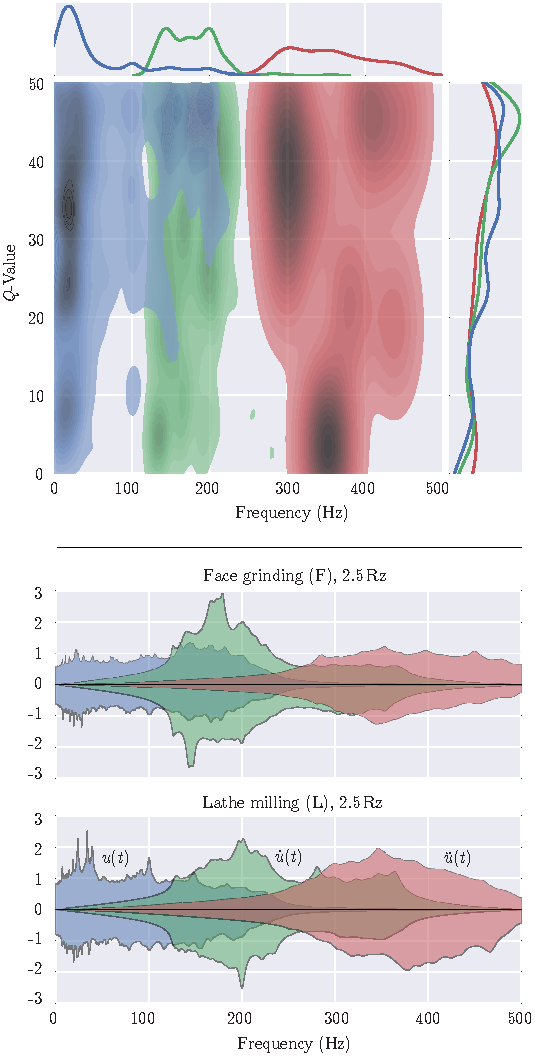
\includegraphics[width=0.4\textwidth]{touch-5}    
    \caption{\label{fig:touch-filters} Visualizing the network in the frequency domain. Frequencies are $0 - 250$, $125 - 375$, or $250 - 500$\,Hz, depending on whether each hidden neuron is encoding a dimension from $u(t)$ (blue), $\dot{u}(t)$ (green), or $\ddot{u}(t)$ (red). (Top) Distribution of bandpass filter parameters from (\ref{eq-bandpass}), weighted by the $\ell^2$-norm of SVM coefficients, and smoothed by a kernel density estimate \cite{michael_waskom_2015_19108}. 
The smallest weights are omitted to reduce visual clutter. Histograms along the sides flatten the distribution across their corresponding axes. (Bottom) Power of bandpass filters per texture (only two shown), weighted by their squared SVM coefficients (unitless). Negatively rectified dimensions are flipped about the $x$-axis for visualization.}
\end{figure}

To evaluate the system, the trained network was tested on each $1$\,s of test data. The 18-dimensional score vector was decoded from the spiking activity of the output population, lowpass filtered with default time constant ($5$\,ms), and sampled every $1$\,ms (see Fig. \ref{fig:touch-raster}). A total score for each texture was obtained by summing together the individual score vectors across the test segment. The classification for each test segment was taken to be the texture with the highest total score. These results are broken down by texture in Table \ref{tab:touch-results}, averaged across each test segment from all four folds, with an overall accuracy of $65.6\%$. The most common classification is the correct texture, in all cases.

By analyzing the trained network, we may succinctly characterize what each classifier is sensitive to in the frequency domain. We visualize this to indicate which bandpass parameters are most important for classifying all textures (see Fig. \ref{fig:touch-filters} top), and which frequencies are most important for classifying a specific texture (see Fig. \ref{fig:touch-filters} bottom). 
The top figure reveals that narrow filters (higher values of $Q$) tend to carry more weight, while frequencies in the range of $50 - 100$, $240 - 260$, and $400 - 500$\,Hz are less useful. The bottom figure shows for example that neurons encoding the negatively rectified dimension of $\dot{u}(t)$ will provide the most evidence for L2.5 when this dimension has power at $200$\,Hz. 

We also compared our approach to a simpler model, 
by training and evaluating the same model without a hidden layer. This baseline model was prepared and validated under the same conditions, except the SVM used the spiking activity of the mechanoreceptor population as its features, rather than the spiking activity from the hidden layer.  Cross-validation accuracy decreased to $17.8\%$, averaged across each test segment from all four folds.
We remark that the baseline still captures temporal information through its various lowpass filters (in the output layer and PSCs) and highpass filters (in the mechanoreceptor cells), yet it is no longer able to isolate particular bands of frequencies. Therefore, it is the addition of bandpass filters in the hidden layer that enable the network to accurately separate the feature space by texture.

\subsubsection{Discussion}

We trained a three-layer network of spiking neurons to classify a set of 18 textures. A biologically plausible model of mechanoreceptors was adapted to encode the input vibrations. Psychophysical experiments and the role of cuneate neurons motivated a hidden layer that extracts frequency information. Lastly, an SVM determined the connection weights into a recurrently connected population. To our knowledge this is a novel semi-supervised approach for classifying dynamic stimuli using a spiking neural network.

A key advantage of our approach is that the network can be simulated in real-time using low-power neuromorphic hardware. At the same time, the NEF endows our model with benefits such as robustness to noise  and parallel computation. Similarly, the system immediately provides classifications online, and performs well with brief inputs lasting only $1$\,s.  These advantages make our method generally suitable for use in robotic applications, thus advancing the state of the art for texture classification. % be more explicit? examples?

A comparison with a baseline model revealed that performance was a consequence of the hidden layer. The first two layers of the network are unsupervised, and so the activity of the hidden layer represents general features that can in theory be reused for other applications. We intend to demonstrate this by extending our system to differentiate between textures, by interpreting the feature vector as a high-dimensional description of a texture. We also suspect that other tasks which process tactile stimuli  can benefit by using this same vector.

Likewise, features of the input stimulus are learned and classified using general techniques from signal processing and machine learning. The methodology that we have described here need not be limited to the use of mechanoreceptor models and bandpass filters. While these tools were needed to appropriately constrain our model, other applications involving the processing of dynamic stimuli (e.g. visual or auditory) may readily place different constraints on how each layer encodes and filters information. This in turn may allow the architecture to be modified and redeployed within other domains. 

The test results indicate how often each texture is confused with another. 
In general, it should be possible to design a simple psychophysical experiment to compare our system to human performance. However, our system is at a fundamental disadvantage since it does not  alter its position or pressure to gather more evidence when unsure of its prediction. We are considering future extensions that solve this issue with a closed-loop system that can actively control its motor movements, with a range of velocities,  based on feedback from the accumulated features.

\subsection{Decoding Filter Optimization}

Include method of simultaneously solving for decoders and linear filter in a single least-squares problem

\subsection{Dale's Principle}

Compare my DalesSolver to Parisian Transform


\section{Biological Detail}

\subsection{Conductance-Based Synapses}

Summarize Andreas' research

\subsection{Adaptative Neurons}

Eric's system itendification
Subtractive adaptation and perfect cancellation
Divisive adaptation (adaptive threshold) and modelling it by the latter
Interpretation in terms of PSC code / objective function, and dimensionality

\subsection{Wilson Neurons}

Peter's work

\subsection{Baal Neurons}

Peter's work


